\documentclass{poly}
\usepackage{main}

\title{Probabilités conditionnelles et indépendance d'événements}
\date{}
\author{Première Spécialité Mathématiques}

\begin{document}
\maketitle

\section{Rappel : Vocabulaire des probabilités}
\textbf{Un joueur ou une joueuse lance deux dés à six faces équilibrés, et observe la somme des valeurs obtenues.}
\begin{definition}
\hfill
\begin{itemize}
\item Une telle situation où le résultats possibles sont connus, mais où l'issue n'est a priori pas décidée à l'avance est nommée \textbf{Expérience aléatoire}.
\item L'ensemble des \textbf{issues} possible de cette expérience est nommé l'\textbf{univers}, habituellement noté $\Omega$. (Ici, un univers envisageable pour cette expérience est $\Omega = \{2;3;4;5;6;7;8;9;10;11;12\}$)
\item Un sous-ensemble de l'univers $\Omega$ est appelé \textbf{événement}. (Par exemple, l'événement correspondant à obtenir une somme paire serait $A = \{2;4;6;8;10;12\}$)
\end{itemize}
\end{definition}
\begin{definition}
Soient $A$ et $B$ deux événements d'une expérience aléatoire d'univers $\Omega$.
\begin{itemize}
\item Si $A = \Omega$, $A$ est appelé \textbf{événement certain}. (Par exemple, obtenir une somme inférieure à $13$ à l'aide de deux dés est un événement certain)
\item Si $A = \emptyset$ (l'ensemble vide), alors $A$ est appelé \textbf{événement impossible}. (Par exemple, obtenir $1$ à l'aide de deux dés est un événement impossible)
\item L'\textbf{union} des événements $A$ et $B$, noté $A \cup B$, se lisant \og $A$ \textbf{union} $B$\fg, est l'événement réalisant les issues de $A$ \textbf{ou} celles de $B$. (Par exemple, si $A = \{4;10\}$ et $B = \{10;12\}$, alors leur union est donnée $A \cup B = \{4;10;12\}$)
\item L'\textbf{intersection} des événements $A$ et $B$ noté $A \cap B$, se lisant \og $A$ \textbf{inter} $B$, est l'évenement réalisant à la fois les issues de $A$ \textbf{et} celles de $B$. (Par exemple, si $A = \{4;10\}$ et $B = \{10;12\}$, alors leur intersection est donnée par $A \cap B = \{10\}$)
\item Le complémentaire de l'événement $A$ noté $\overbar{A}$, se lisant \og $A$ \textbf{barre}\fg, est l'événement réalisant toutes les issues qui ne sont pas réalisées par $A$. (Par exemple, le complémentaire de l'évenement correspondant à obtenir une somme paire serait l'événement correspondant à obtenir une somme impaire)
\end{itemize}
\end{definition}
\begin{center}
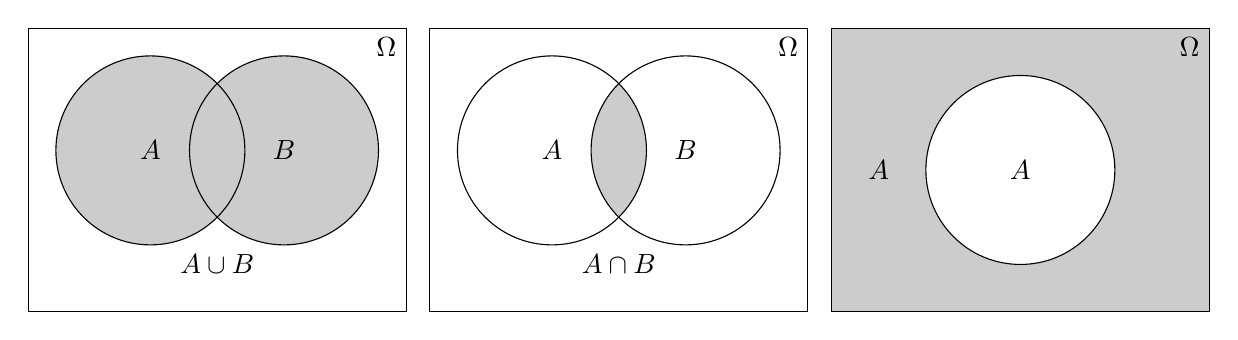
\begin{tikzpicture}[scale = 0.6]
\draw (-4,-2) rectangle (4,4) node[below left] {$\Omega$};
\begin{scope}
\clip (135:2) circle (2);
\fill[color=gray!40] (45:2) circle (2);
\end{scope}
\draw (135:2) node{$A$} circle (2);
\draw (45:2) node{$B$} circle (2);
\draw (0,-1) node{$A \cap B$};
\begin{scope}[xshift=-8.5cm]
\draw (-4,-2) rectangle (4,4) node[below left] {$\Omega$};
\fill[color=gray!40] (135:2) circle (2);
\fill[color=gray!40] (45:2) circle (2);
\draw (135:2) node{$A$} circle (2);
\draw (45:2) node{$B$} circle (2);
\draw (0,-1) node{$A \cup B$};
\end{scope}
\begin{scope}[xshift=8.5cm]
\fill[color=gray!40] (-4,-2) rectangle (4,4);
\draw (-4,-2) rectangle (4,4) node[below left] {$\Omega$};
\fill[color=white] (0,1) circle (2);
\draw (0,1) circle (2) node {$A$};
\draw (-3,1) node {$\overbar{A}$};
\end{scope}
\end{tikzpicture}   
\end{center}
\begin{example}
Proposer deux événements $A$ et $B$ dont l'intersection et l'union sont non-vide.

\end{example}
\newpage
\begin{definition}
Soient $A$ et $B$ deux événements d'une expérience aléatoire d'univers $\Omega$. Alors $A$ et $B$ sont \textbf{disjoints} si et seulement si $A \cap B = \emptyset$.
\end{definition}
\begin{definition}
Soit une expérience aléatoire d'univers $\Omega$. Une \textbf{probabilité} sur $\Omega$ associe à tout événement $A$ un nombre réel $P(A)$ compris entre $0$ et $1$, et vérifie deux propriétés :
\begin{itemize}
\item $P(\Omega) = 1$
\item $P(A \cup B) = P(A) + P(B)$ si les événements $A$ et $B$ sont disjoints.
\end{itemize}
\end{definition}
\begin{example}
Si $A$ est l'événement consistant à obtenir $7$ aux dés, alors
\begin{equation*}
P(A) = \dfrac{1}{6}
\end{equation*}
\end{example}
\begin{definition}
\textbf{Établir la loi de probabilité} d'une expérience aléatoire d'univers $\Omega$ consiste à associer à chaque issue $w \in \Omega$ sa probabilité $P(\{w\})$.
\end{definition}
\begin{remark}
\textbf{Ainsi, si la loi de probabilité est connue, la probabilité d'un événement $P(A)$ est donnée par la somme de toutes les probabilités des issues réalisant $A$.}
\end{remark}
\begin{example}
On donne la loi de probabilité concernant la somme de deux dés.
\begin{equation*}
\begin{tblr}{hlines, vlines, row{2} = {0.8cm}, columns={c}, column{1} = {l}}
w \in \Omega & 2 & 3 & 4 & 5 & 6 & 7 & 8 & 9 & 10 & 11 & 12\\
P(\{w\}) & \dfrac{1}{36} & \dfrac{1}{18} & \dfrac{1}{12} & \dfrac{1}{9} & \dfrac{5}{36} & \dfrac{1}{6} & \dfrac{5}{36} & \dfrac{1}{9} & \dfrac{1}{12} & \dfrac{1}{18} & \dfrac{1}{36}\\
\end{tblr}
\end{equation*}
\begin{alphaquestions}
\item Vérifier que la somme des probabilités vaut $1$. 
\item En déduire la probabilité de l'événement $B$ \og La somme des dé est paire\fg.
\end{alphaquestions}

\end{example}
\begin{definition}
Soit une expérience aléatoire d'univers $\Omega$, et $P$ une probabilité sur $\Omega$. On est en \textbf{situation d'équiprobabilité} si la loi de probabilité de $P$ associe la même valeur à toutes les issues.
\end{definition}
\begin{example}
\hfill
\begin{itemize}
\item Regarder le résultat du lancer d'un unique dé équilibré est une expérience aléatoire en situation d'équiprobabilité.
\item Regarder la somme du résultat de deux dé équilibrés n'est pas une expérience aléatoire en situation d'équiprobabilité.
\end{itemize}
\end{example}
\begin{proposition}
Soit une expérience aléatoire d'univers $\Omega$ non vide, \textbf{en situation d'équiprobabilité}, et soit $A$ un événement d'$\Omega$. Alors la probabilité de $A$ est donnée par
\begin{equation*}
P(A) = \dfrac{\text{Nombre d'éléments de $A$}}{\text{Nombre d'éléments de $\Omega$}}
\end{equation*}
\end{proposition}
\newpage
\section{Représentation d'expérience aléatoire}
\subsection{Arbres pondérés}
Un \textbf{arbre pondéré de probabilités} permet de représenter des événements \textbf{successifs} d'une expérience aléatoire. 
\begin{example}
Dans une urne, il y a quatre boules bleues et deux boules rouges. On tire successivement deux boules \textbf{sans remise} (on ne remet pas la première boule dans l'urne). On s'interroge sur la probabilité de tirer une boule rouge au deuxième tirage.

Pour cela, on représente l'expérience à l'aide d'un arbre pondéré de probabilité :
\begin{center}
\begin{tikzpicture}[scale=1.2]
\node (A) at (2,1) {Rouge};
\node (AB) at (4,1.5) {Rouge};
\node (ABn) at (4,0.5) {Bleu};
\node (An) at (2,-1) {Bleu};
\node (AnB) at (4,-0.5) {Rouge};
\node (AnBn) at (4,-1.5) {Bleu};
\draw (0,0) -- (A) node[above,midway] {$\dfrac{2}{6}$} -- (AB) node[midway,above] {$\dfrac{1}{5}$};
\draw (A) -- (ABn) node[midway,below] {$\dfrac{4}{5}$};
\draw (0,0) -- (An) node[midway,below] {$\dfrac{4}{6}$} -- (AnB) node[above,midway] {$\dfrac{2}{5}$};
\draw (An) -- (AnBn) node[below,midway] {$\dfrac{3}{5}$};    
\end{tikzpicture}
\end{center}
\end{example}
\begin{proposition}
\hfill
\begin{itemize}
\item Une branche de la racine à une extrémité correspond à l'intersection des événements associés. Pour calculer la probabilité de cette intersection, il faut multiplier les probabilités sur la branche. 
\item La somme de toutes les probabilités issues d'un même noeud vaut $1$.
\item La probabilité d'un événement est égale à la somme des probabilités de toutes les branches contenant cet événement. 
\end{itemize}        
\end{proposition}

\begin{exercize}
En reprenant l'expérience décrite précédemment et l'arbre pondéré associé, répondre aux questions suivantes :
\begin{alphaquestions}
\item Soit $A$ : \og Les deux boules tirées sont rouges \fg. Calculer $P(A)$.
\item Soit $B$ : \og Les deux boules tirées sont de couleur différentes \fg. Calculer $P(B)$
\end{alphaquestions}
\end{exercize}

\begin{remark}
\hfill
\begin{itemize}
\item Chaque noeud de l'arbre représente un événement. La racine est un noeud correspondant à l'événement $\varnothing$.
\item Les branches issues d'un noeud correspondent aux événements possibles de survenir une fois que l'événement du noeud est réalisé. Par exemple, une fois que l'on a tiré une boule rouge, il est \textbf{possible} de tirer une seconde boule rouge ou une boule bleue.
\item Un arbre a une certaine \og hauteur \fg, correspondant aux nombre d'étapes successives dans l'expérience. Par exemple, l'arbre est de hauteur $2$ parce qu'il y a deux tirages successifs dans l'urne. 
\end{itemize}
\end{remark}

\newpage
\subsection{Tableau}

Certaines expériences aléatoires se prêtent bien à l'utilisation de tableaux à double entrée. C'est le cas des expériences où l'on regarde deux événements \textbf{simultanés}.
\begin{example}
La somme du résultat du lancer de deux dés (un dé bleu et un dé rouge) est un bon exemple, car il peut être résumé comme ceci :
\begin{equation*}
\begin{tblr}{hlines,vlines}
\diagbox{Rouge}{Bleu}&1&2&3&4&5&6\\
1&2&3&4&5&6&7\\
2&3&4&5&6&7&8\\
3&4&5&6&7&8&9\\
4&5&6&7&8&9&10\\
5&6&7&8&9&10&11\\
6&7&8&9&10&11&12\\
\end{tblr}
\end{equation*}
Puisque toutes les cases correspondent à des situations équiprobables, il devient très facile de calculer la probabilité d'obtenir la somme de votre choix.
\end{example}

\begin{exercize}
\hfill
\begin{alphaquestions}
\item Calculer la probabilité que la somme obtenue soit 5.
\item Calculer la probabilité que la somme obtenue soit paire.
\end{alphaquestions}
\end{exercize}

\begin{example}
Dans un lycée, on interroge les filles et les garçons sur leur préférence d'activité extrascolaire.

\begin{center}
\begin{tblr}{hlines, vlines, columns = {c}}
\diagbox{Activité}{Genre}&Fille&Garçon\\
Artistique&$450$&$370$\\
Sportive&$850$&$230$\\
\end{tblr}
\end{center}
\end{example}

\begin{exercize}
On interroge un élève de ce lycée au hasard.
\begin{alphaquestions}
\item Quelle est la probabilité que l'élève interrogé soit un garçon qui préfère une activité artistique ?
\item Quelle est la probabilité que l'élève interrogé soit une fille ?
\item On interroge une fille. Quelle est la probabilité que l'élève interrogée préfère une activité sportive ?
\end{alphaquestions}
\end{exercize}

\begin{remark}
\hfill
\begin{itemize}
\item Une case correspond donc à l'intersection de deux événements.
\item Le nombre total d'issues dans chaque événement dépend du contexte. Dans le cas des dés, le nombre de cases du tableau donne le nombre total d'issues. Dans l'exemple du lycée, le nombre total d'issues est donné par le nombre total d'élève, et est obtenu en faisant la somme du nombre d'effectifs de chaque case.
\end{itemize}
\end{remark}

\newpage

\section{Théorie des probabilités}
\subsection{Probabilités conditionnelles}

\begin{definition}
Soit une expérience aléatoire d'univers $\Omega$, et $A$ et $B$ deux événenements de $\Omega$. On suppose de plus que $P(A) \neq 0$.

Alors, la \textbf{probabilité de $A$ sachant $B$}, notée $P_{A}(B)$, est la probabilité que $B$ se réalise \textbf{sachant} que $A$ s'est déjà réalisé.
\end{definition}

\begin{example}
Une usine produit des vis et des clous. Certaines pièces ont une défaut de fabrication. On prend une pièce produite par cette usine au hasard.

On note $V$\og La pièce choisie est une vis\fg et $D$\og La pièce choisie a un défaut de fabrication\fg. Dans chacune des situations suivantes, donner la probabilité correspondante (en choisissant bien la bonne notation)

\begin{alphaquestions}
\item Il y a $4\%$ de vis présentant un défaut de fabrication parmi toutes les pièces produites par l'usine.
\item Il y a $2\%$ de vis présentant un défaut de fabrication parmi les vis produites par l'usine.     
\end{alphaquestions}
\vspace*{0.5cm}

\end{example}

\begin{proposition}[Formule des probabilités composées]
Soit $A$ et $B$ deux événements de $\Omega$ tels que $P(A) \neq 0$. Alors 
\begin{equation*}
P(A \cap B) = P(A) \times P_A(B)
\end{equation*}
\end{proposition}

\begin{remark}
Il s'agit de la règle de calcul de la probabilité d'une seule branche dans un arbre pondéré.
\end{remark}

\begin{proposition}
Soit $A$ et $B$ deux événements de $\Omega$ tels que $P(A) \neq 0$. Alors 
\begin{equation*}
P_A(B) = \dfrac{P(A \cap B)}{P(A)}
\end{equation*}
\end{proposition}
\begin{example}
On tire une bille au hasard dans un sac. Chaque bille est grosse ou petite, et chaque bille est rouge ou verte. On note $R$ \og La bille est rouge\fg, et $G$ \og la bille est grosse \fg. Alors le tableau suivant donne la répartition du sac.
\begin{equation*}
\begin{tblr}{hlines,vlines,columns = {c}}
\diagbox{Taille}{Couleur}&R&\overbar{R}&\text{Total}\\
G&12&8&20\\
\overbar{G}&7&13&20\\
\text{Total}&19&21&40\\
\end{tblr}
\end{equation*}
\begin{alphaquestions}
\item Quelle est la probabilité d'obtenir une grosse bille rouge ?
\item Quelle est la probabilité d'obtenir une petite bille, sachant que la bille tirée est verte ?
\end{alphaquestions}
\vspace*{0.5cm}

\end{example}

\newpage
\subsection{Partition de l'univers}
\begin{definition}
Soit une expérience aléatoire d'univers $\Omega$. On dit que des événements $A_1$, $A_2$, \dots $A_n$ forment une \textbf{partition de $\Omega$} si et seulement si
\begin{equation*}
\begin{cases}
A_1 \cup A_2 \cup \dots \cup A_n = \Omega\\
\text{$A_1$, $A_2$ \dots $A_n$ sont disjoints deux à deux} 
\end{cases}
\end{equation*}
\end{definition}
\begin{remark}
\hfill
\begin{itemize}
\item Créer une partition de $\Omega$, c'est regrouper chaque issue de $\Omega$ dans un unique paquet.
\item Soit $A$ un événement de $\Omega$, alors $A$ et $\overbar{A}$ forment une partition de $\Omega$. 
\end{itemize}
\end{remark}

\begin{example}
On considère le lancer d'un seul dé équilibré. Alors si $A$\og le résultat est pair\fg, $B$\og le résultat est $1$\fg et $C$ \og le résultat est impair supérieur ou égal à $3$\fg, on en déduit que $A$, $B$ et $C$ forment une partition de l'univers de l'expérience.
\end{example}

\begin{proposition}[formule des probabilités totales]
Soit $B$ un évenement, et $A_1$, $A_2$, \dots, $A_n$ une partition de $\Omega$. Alors,
\begin{equation*}
P(B) = P(B \cap A_1) + P(B \cap A_2) + \dots + P(B \cap A_n)
\end{equation*}
\end{proposition}

\begin{remark}
Le schéma suivant permet de visualiser la situation.
\begin{center}
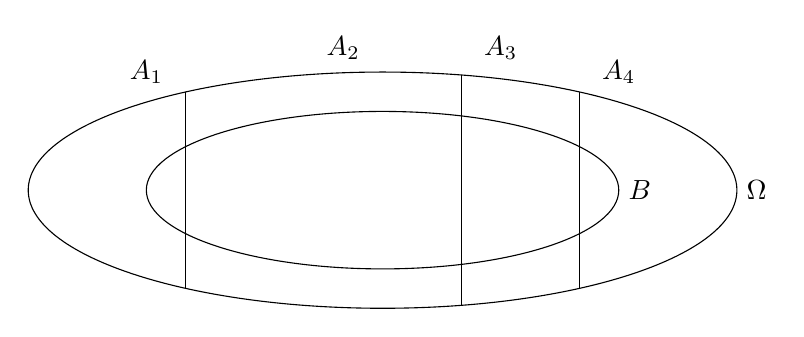
\begin{tikzpicture}
\draw (0,0) ellipse (4.5 and 1.5);
\draw (0,0) ellipse (3 and 1);
\draw (4.5,0) node[right] {$\Omega$};
\draw (3,0) node[right] {$B$};
\draw (-3,1.5) node {$A_1$};
\draw (-0.5,1.8) node {$A_2$};
\draw (1.5,1.8) node {$A_3$};
\draw (3,1.5) node {$A_4$};
\clip (0,0) ellipse (4.5 and 1.5);
\draw (1,1.5) -- (1,-1.5);
\draw (2.5,1.5) -- (2.5,-1.5);
\draw (-2.5,1.5) -- (-2.5,-1.5);
\end{tikzpicture}
\end{center}
\end{remark}

\begin{remark}
La formule des probabilité totale correspond à la méthode de calcul de la probabilité de plusieurs branches d'un arbre pondéré.

À chaque hauteur de l'arbre, il faut donc s'assurer que tous les événements originaires d'une même branche forment une partition de l'univers $\Omega$. 
\end{remark}

\newpage

\section{Indépendance}
\subsection{Indépendance d'événements}

\begin{definition}
Soit une expérience aléatoire d'univers $\Omega$, et $P$ une probabilité sur $\Omega$.

Soit $A$ et $B$ deux événements de $\Omega$. Alors, $A$ et $B$ sont dits \textbf{indépendants} si et seulement si $P(A \cap B) = P(A)P(B)$.
\end{definition}

\begin{example}
On lance deux dés : un dé rouge et un dé bleu. On pose les événements $A$ \og le dé rouge renvoie un résultat pair\fg, et $B$ \og le dé bleu renvoie un résulat supérieur ou égal à $4$\fg. Les événements $A$ et $B$ sont-ils indépendants ?
\vspace*{0.5cm}

\end{example}
\begin{proposition}
Soit $A$ et $B$ deux événements, tels $P(A) \neq 0$. Alors, si $A$ et $B$ sont indépendants, on a
\begin{equation*}
P_A(B) = P(B)
\end{equation*}
\end{proposition}
\begin{remark}
Quand deux événements sont indépendants, cela signifie que la réalisation de l'un n'a pas d'influence sur la réalisation de l'autre.

À ne pas confondre avec des événements \textbf{incompatibles} ($P(A \cap B) = 0$).
\end{remark}
\begin{proof}
Voir cahier.

\end{proof}
\begin{proposition}
Soit $A$ et $B$ deux événenements indépendants de $\Omega$. Alors $\overbar{A}$ et $B$ sont indépendants.
\end{proposition}
\begin{proof}
Voir cahier.
\end{proof}

\subsection{Succession d'expériences indépendantes}
\begin{remark}
Quand on réalise successivement deux expériences aléatoires telles que les événements de la premières sont tous indépendants avec ceux de la seconde, on dit que l'on réalise une \textbf{succession d'expériences indépendantes}. 

Autrement dit, deux expériences aléatoire sont dites indépendantes quand le résultat de la première n'a pas d'influence sur le résultat de la seconde.
\end{remark}

\end{document}